%%%%%%%%%%%%%%%%%%%%%%%%%%%%%%%%%%%%%%%%%%%%%%%%%%%%%%%%%%%%%%%%%%
%%%%%%%% ICML 2015 EXAMPLE LATEX SUBMISSION FILE %%%%%%%%%%%%%%%%%
%%%%%%%%%%%%%%%%%%%%%%%%%%%%%%%%%%%%%%%%%%%%%%%%%%%%%%%%%%%%%%%%%%

% Use the following line _only_ if you're still using LaTeX 2.09.
%\documentstyle[icml2015,epsf,natbib]{article}
% If you rely on Latex2e packages, like most moden people use this:
\documentclass{article}

% ams packages
\usepackage{amsmath,amsfonts,amssymb}

% use Appendix
\usepackage{appendix}

\usepackage{multicol}

% use Times
\usepackage{times}
% For figures
\usepackage{graphicx} % more modern
%\usepackage{epsfig} % less modern
\usepackage{subfigure} 

% For citations
\usepackage{natbib}

% For algorithms
\usepackage{algorithm}
\usepackage{algorithmic}

% As of 2011, we use the hyperref package to produce hyperlinks in the
% resulting PDF.  If this breaks your system, please commend out the
% following usepackage line and replace \usepackage{icml2015} with
% \usepackage[nohyperref]{icml2015} above.
\usepackage{hyperref}

% Packages hyperref and algorithmic misbehave sometimes.  We can fix
% this with the following command.
\newcommand{\theHalgorithm}{\arabic{algorithm}}

% Employ the following version of the ``usepackage'' statement for
% submitting the draft version of the paper for review.  This will set
% the note in the first column to ``Under review.  Do not distribute.''
%\usepackage{icml2015} 

% Employ this version of the ``usepackage'' statement after the paper has
% been accepted, when creating the final version.  This will set the
% note in the first column to ``Proceedings of the...''
\usepackage[accepted]{icml2015}


% The \icmltitle you define below is probably too long as a header.
% Therefore, a short form for the running title is supplied here:
\icmltitlerunning{10-708 PGM Project Final Report: Learning SNP-Gene Network Using Mixed Graphical Model}

\begin{document} 

\twocolumn[
\icmltitle{10-708 PGM Project Final Report \\ 
           Learning SNP-Gene Network Using Mixed Graphical Model}

% It is OKAY to include author information, even for blind
% submissions: the style file will automatically remove it for you
% unless you've provided the [accepted] option to the icml2015
% package.
\icmlauthor{Hyun Ah Song}{hyunahs@andrew.cmu.edu}
\icmladdress{Machine Learning Department, Carnegie Mellon University, Pittsburgh, PA 15213}
\icmlauthor{Ji Oh Yoo}{jiohy@andrew.cmu.edu}
\icmladdress{Computer Science Department, Carnegie Mellon University, Pittsburgh, PA 15213}

% You may provide any keywords that you 
% find helpful for describing your paper; these are used to populate 
% the "keywords" metadata in the PDF but will not be shown in the document
\icmlkeywords{boring formatting information, machine learning, ICML}

\vskip 0.3in
]

\section{Introduction}
Recent progress on large scale genome-wide studies show that many human common diseases, including diabetes, asthma, and cancer, consist of complex reactions of proteins, which are controlled by regulatory networks and are expressed from highly correlated genetic variations \cite{basso2005reverse, chen2008variations}. Thus, rather than simple correlation studies between a few clinical phenotypes and genetic variations of interest, discovering of eQTL mapping between the multiple genetic variations and multiple disease-related proteins' expression rates is necessary to analyze the occurrence mechanism of the diseases and the functional roles of those proteins in the mechanism. This requires the joint learning of the genetic variations and the expression of the related proteins rather than combining the results from the independent study on each genome or phenome. Multiple regression studies have been conducted to identify these mappings between single-nucleotide polymorphisms (SNPs) and related gene expression rates, and to develop the more efficient and accurate methods for this eQTL mappings discovery \cite{kim2010tree, sohn2012joint}. We adopted conditional undirected mixed graphical model \cite{lee2013structure} for SNP-gene network learning to relax the assumptions and lessen requirements for learning in the previous methods, and analyzed the performance of our model in both synthetic environment and real-world application.




\section{Background \& Related Work}
\label{LiteratureReview}


\subsection{Related Work}
There have been various types of solutions to the problem of learning SNPs-gene network. One popular solution is to solve the problem as multiple-output regression, a straight-forward extension of single-output regression. 
Given SNPs information as inputs, multiple-output regression tries to solve the regression task for each output simultaneously while sharing the coefficient matrix for all the tasks. It can incorporate L-1 penalty (lasso) for sparse model and L-21 mixed penalty for desired sparsity pattern in the coefficient matrix \cite{obozinski2008high}.




Tree-guided group lasso, or GFlasso was proposed by Kim and coworkers \cite{kim2010tree}.
GFlasso aims to learn the common set of inputs for each cluster of outputs, using group lasso penalty and systematic weighting scheme for inputs, where inputs are grouped together to be mapped to the outputs, and output clusters with strong correlation are guided to share common input groups.
GFlasso requires the prior knowledge of output tree structure, which is not always possible.
Also, the weighting scheme of guiding the common set of inputs for highly correlated clusters is such a strong assumption that may not be true in reality.


An algorithm called multivariate regression with covariance estimation (MRCE) that aims to learn both multivariate regression parameters and the correlation of outputs was introduced by Rothman and coworkers \cite{rothman2010sparse}.
By regularizing regression parameter and correlation matrix separately, the MRCE solve bi-convex problem, which may not lead to the global optimum. Although MRCE is favorable in a way that it learns the output structure, MRCE does not force structured sparsity when learning regression parameters for inputs, which is an important property when dealing with SNPs-gene data.


An algorithm that bring together the advantages of the two previous works \cite{kim2010tree} \cite{rothman2010sparse} was introduced by Sohn and coworkers \cite{sohn2012joint}. 
The proposed algorithm jointly learns regression parameters and output structure with constraint of structure sparsity in inputs, by learning conditional Gaussian graph model.
Although proposed algorithm resolves the main problems in previous studies, it assumes that input and output are treated as continuous data, which is not true for SNPs-gene data.
Therefore, it leaves some space for further refinement of the assumptions used in this algorithm.









In order to solve the problem in more natural way, we can adopt 'mixed graphical models' into our problem.
Mixed graphical models refer to graphical models that allow for both discrete and continuous variables.


Lauritzen first proposed a mixed graphical model for variables of both discrete and continuous \cite{lauritzen1989graphical}.
 Although this mixed graphical model is carefully designed for general cases, this makes resulting conditional distribution complex. Also, the mean and covariance matrices exist for every possible configurations of states of discrete variables, which results in exponential increase in number of parameters to learn depending on the number of discrete variables.




Later by Jason and coworkers, the mixed graphical model was further developed into more simplified and intuitive version \cite{lee2013structure}. 
The authors proposed a mixed graphical model that provides intuitive forms of conditional distributions: conditional distribution of a discrete variable reduces to multi-class logistic regression, and that of a continuous variable to Gaussian linear regression. 
By making assumptions on the general mixed graphical models  \cite{lauritzen1989graphical}, proposed algorithm scales up more efficiently: it has common covariance matrix, and additive mean.


To our knowledge, there has not been any study that learns the SNP-gene network as multi-task regression problem using mixed graphical models. 
In this project, we would like to extend the basic concepts proposed by Sohn  \cite{sohn2012joint} using mixed graph models \cite{lee2013structure}, to solve the problem in more natural way.







\subsection{Background}
One of the most commonly used method in estimation of SNP-gene network is the multiple-output extension of single-output regression method with lasso penalty \cite{tibshirani1996regression}, which solves the following optimization problem.

\begin{align}\label{eq:lasso}
\text{arg} \min_{\textbf{B}} \text{tr}((\mathbf{Y}-\mathbf{XB})(\mathbf{Y}-\mathbf{XB})^T) + \lambda \| \mathbf{B}\|_1,
\end{align}

where $\mathbf{X}=(\mathbf{x_1}, ... ,\mathbf{x_N})^T$, $\mathbf{Y}=(\mathbf{y_1}, ... ,\mathbf{y_N})^T$ are input and output data, and $\mathbf{x_i}=(x_{i1}, ... ,x_{iJ})^T \in \mathbb{R}^J$, and $\mathbf{y_i}=(y_{i1}, ... ,y_{iK})^T \in \mathbb{R}^K$.
The output is estimated by regression: $\mathbf{y_i}=\mathbf{Bx_i}+\mathbf{\varepsilon_i}$, where $\varepsilon  \sim \mathcal{N}(0, \mathbf{\Psi})$.
By enforcing sparsity in \textbf{B}, it is able to take into account of the problem setting that we have $J >> N$, where the number of SNPs is higher than the number of samples. Also, using L-1/L-2 mixed norm penalty can be used for joint feature selection \cite{obozinski2008high}.


Despite the simple formulation and optimization method for multiple-output regression, it does not capture the relatedness among the output variables in the data. To address this problem of learning structured sparsity and structure in output variables, Graph-guided Fused Lasso is developed with fusion penalty according to pre-computed degree of relatedness among the output \cite{kim2009statistical}, but it needs prior knowledge of the data, which can differ by each problem setting and its problem domain. To overcome this problem of necessity of prior knowledge, Sohn and coworkers proposed Sparse Conditional Gaussian Graphical Model, which extends the problem of learning standard regression model into learning a conditional Gaussian graphical model \cite{sohn2012joint}. It assumes that the joint distribution of input and output as a single multivariate Gaussian distribution as Eq. \ref{eq:jointG}.

\begin{align}\label{eq:jointG}
\begin{split}
\begin{bmatrix}
    \mathbf{x_i}\\
    \mathbf{y_i}
\end{bmatrix}
 \sim \mathcal{N}
 \begin{pmatrix}
\begin{bmatrix}
    \mathbf{0}_J  \\
   \mathbf{0}_K
\end{bmatrix}
,
    \Sigma
\end{pmatrix} \\
\mathbf{\Sigma}^{-1}= \begin{pmatrix}
    \mathbf{\Theta}_{xx} & \mathbf{\Theta}_{xy}\\
   \mathbf{\Theta}_{xy}^T &  \mathbf{\Theta}_{yy}  
\end{pmatrix}
\end{split}
\end{align}
Then, the parameters $\Theta$ and $\Phi$ in Eq. \ref{eq:lasso} can be reconstructed by $\mathbf{B}=\mathbf{\Sigma}_{xy}^T \mathbf{\Sigma}_{xx}^{-1}=-\mathbf{\Theta}_{yy}^{-1}\mathbf{\Theta}_{xy}^T$, and $\mathbf{\Psi}= \mathbf{\Theta}_{yy}^{-1}$.

Although this method by Sohn suits the needs for the SNP-gene network estimation problem as it learns both structured sparsity in $\Theta$ and output structure in $\Phi$, and formulates the problem using the standard regression problem, the underlying assumption is that both input and output data constitute of continuous variables. This assumption is from that the degree of genetic variation, the deviation from major alleles, can be measured by the number of minor alleles in a person's genotype, and the relationship between the deviation and output is linear. However, the phenotypes from genes with 0 or 1 minor alleles can be drastically different from those of 2 minor alleles in many cases including examples from Mendel's Law.  Thus, it is reasonable approach to relax this assumption in the previously developed regression models and model the SNPs as categorical, discrete values.

As with the previous models, continuous variables can be modeled as a multivariate Gaussian: $y \sim \mathcal{N}(0, \Theta^{-1})$, where the inverse covariance matrix $\Theta$ can be estimated via graphical lasso. For discrete variables, pairwise Markov random field $p(x) \propto exp \sum_{r\leq j} \phi_{rj}(x_r, x_j)$ is one of the commonly used graphical model.
Studies on mixed graphical model, which combines two commonly used graphical models of Gaussian and pair-wise graphical models so that it can handle data consisting of both continuous and discrete variables, have been conducted by Lauritzen and coworkers, where the conditional distribution is modeled as $p(y|x) = \mathcal{N}(\mu(x), \Sigma(x))$ \cite{lauritzen1989graphical}.
Despite of the novelty and specific applications of the mixed graphical model, it has not been used as widely due to its complexity in learning the parameters, and lack of intuition when derived to the other types of distributions.

Lee and coworkers \cite{lee2013structure} have proposed a special case of the mixed graphical model that resolves the problem of the complexity in parameter learning and vague forms of derived distributions by making several assumptions.
 The detailed explanation follows in section \ref{Methods}.
 
In our work, we investigate the performance of conditional mixed graphical model, whose assumption on the types of data it can handle does not violate our problem setting for SNP-gene network estimation. We compare the performance of the mixed graphical model when applied to SNP-gene network estimation problem, and that of commonly used method.


\section{Methods}
\label{Methods}
Our goal is to improve the method of learning SNP-gene network by adopting the conditional undirected mixed graphical model in which we can embed both discrete variables for SNPs and continuous variables for gene expression rates.

\subsection{Baseline Method}
Lee and coworkers \cite{lee2013structure} proposed a mixed graphical model of discrete and continuous variables, where the joint distribution is expressed as:

\begin{align}
p(x, y ; \Theta) \propto \exp \Big( &\sum_{k=1}^{q} \sum_{l=1}^{q} \phi_{kl} (x_k, x_l) \nonumber \\
+ \sum_{k=1}^{p} \sum_{s=1}^{q} \rho_{ks}(x_k) y_s  &+ \sum_{s=1}^{p} \alpha_s y_s + \sum_{s=1}^{p} \sum_{t=1}^{q} -\frac{1}{2} \beta_{st} y_s y_t \Big) \label{eq:joint}
\end{align} 

where $x_1, ... x_p$ are discrete variables representing the occurrences for each SNP and $y_1, ..., y_q$ are continuous variables representing the gene expression rate of each gene. 
The parameters are $\Theta = [\{\phi_{kl}\}, \{\rho_{k}\}, \{\alpha_{s}\}, \{\beta_{st}\}]$, where $\phi_{kl}$, $\rho_{k}$, $\alpha_{s}$, $\beta_{st}$ are the discrete-discrete edge potential, continuous-discrete edge potential, continuous node potential, and continuous-continuous edge potential, respectively.

By making further assumptions on mixed graphical models originally introduced in \cite{lauritzen1989graphical}, the mixed graphical model \ref{eq:joint} proposed by Lee \cite{lee2013structure} yields intuitive results when reformulated into various forms of distributions. The conditional distribution of continuous variables and discrete variables given the rest reduces to Gaussian linear regression, and multi-class logistic regression, respectively. Furthermore, when the data consists of continuous and discrete variables only, the model reduces to multivariate Gaussian model, and pairwise discrete Markov random field, respectively. 

\subsection{Revised Method}
We are interested in learning the SNP-gene network structure, and the conditional distribution of the gene expression, given observed SNPs.
Therefore, we only need to focus on learning the conditional distribution of the network rather than learning the full joint distribution. 

The conditional distribution of continuous variables given discrete variables of the mixed graphical model in \cite{lee2013structure} reduces to the form of multivariate Gaussian distribution.

\begin{align}
p(y|x) &= \mathcal{N}(B^{-1}\gamma(x), B^{-1}) \label{eq:cond_prob}\\
\{\gamma(x)\}_s &= \alpha_s + \sum_{k} \rho_{ks}(x_k) \\
p(x) &\propto \exp \Big( \sum_{k} \sum_{l} \phi_{kl}(x_k, x_l) + \frac{1}{2} \gamma(x))^\intercal B^{-1} \gamma(x) \Big)
\end{align}

where $B$ is a symmetric, positive definite inverse covariance matrix $B = \{ \beta_{st}\}$ that is shared across the Gaussian distributions. 

From the property of multivariate Gaussian distribution, the log likelihood of the parameters $\Theta$ given discrete variables $y$ can be expressed as:
\begin{align}
\log p(y | x; \Theta) &= -\frac{1}{2}\log |B^{-1}| -\frac{k}{2} (2 \pi) \nonumber    \\
& -\frac{1}{2} (y - B^{-1} \gamma(x)^\intercal B (y - B^{-1} \gamma(x)) \label{eq:loglikli} \\ 
l_p(\Theta) &= -\frac{1}{2} tr\Big((Y - B^{-1} \Gamma(X))^\intercal B (Y - B^{-1} \Gamma(X)) \Big) \nonumber \\
& -\frac{N}{2} \log|B^{-1}| + \lambda_1 \|\{\beta_{st}\}\|_1 + \lambda_2 \|\{\rho_{ks}\}\|_1 \label{eq:obj}
\end{align}

The parameter $\Theta^*$ that minimizes this L-1 penalized log-likelihood will give us a sparse and consistent estimator, and by comparing the parameters with results in multi-task regression settings, we can analyze the existence of direct and indirect relationship between SNPs and gene expression rates.

For the parameter estimation, we minimize the negative log-likelihood expressed in product of each variable given the rest as follows:
\begin{align}
\tilde{l}(\Theta |y) = - \sum_{s=1}^{p} \log p(y_s |y_{\setminus s}, x;\Theta),
\end{align}
where from \ref{eq:joint}, $p(y_s |y_{\setminus s}, x;\Theta)$ can be reformulated as follows:
\begin{align}
&p(y_s |y_{\setminus s}, x;\Theta) =\nonumber    \\
& \frac{\sqrt{\beta_{ss}}}{\sqrt{2\pi}} \exp \left(\frac{-\beta_{ss}}{2} \left(y_s - \frac{\alpha_s + \sum_j \rho_{sj}(y_j)-\sum_{t=s}\beta_{st}y_t }{\beta_{ss}}\right) \right)^2
\end{align}




\subsection{Optimization}
For the optimization, proximal Newton method \cite{schmidt2010graphical,schmidt2011projected} is used. Proximal Netwon optimization method breaks down the optimization problem into $f(x) + g(x)$, where $f(x)$ is smooth and convex function, and $g(x)$ is a convex function, but not necessarily smooth. 
In our problem, functions $f(x)$ and $g(x)$ correspond to the negative log-likelihood and sparsity constraint, respectively.

Proximal Newton method is an extension of proximal gradient method that considers the second order information of $f(x)$ instead of the first order.
The proximal gradient seeks next point by computing $x_{k+1} = prox_t (x_k - t \bigtriangledown(x_k))$, where $prox_t(x)=\text{argmin}_u(\frac{1}{2t}{\|x-u\|}^2 + g(u))$, and $t$ is chosen by Armijo line search algorithm. In proximal Newton method, $Hprox$ is used, where the $prox$ operator is extended to $\| \cdot \|_H$, where $H=\bigtriangledown^2 f(x_k)$. For each iteration, proximal Newton method finds the next point that minimizes below function.
\begin{align}
  &\bigtriangledown f(x_k)^T(u-x_k)+\frac{1}{2t}(u+x_k)^TH(u-w_k)+g(u) \nonumber    \\
 & =  Hprox_t(x_k-tH^{-1}\bigtriangledown f(x_k)).
\end{align}

Previous studies on proximal Newton method \cite{lee2012proximal} shows that it converges faster especially when $n$ is large, with better accuracy compared to the proximal gradient method.

For the implementation, $H$ is approximated using BFGS.
We used PNOPT package \cite{lee2012proximal} for implementation of proximal Newton optimization algorithm.



\section{Experiments}
We compare the performance of our method to lasso, multi-task lasso with $L_1/L_2$ regularization, and sparse CGGM using synthetic dataset and will compare the performances on real dataset for eQTL mapping later.

\subsection{Basic Synthetic Experiments}
We analyze the performance of our method on the synthetic dataset. We created a simple model as a ground truth with 10 discrete variables (input) and 10 continuous variables (output). The discrete variables have two possible binary states, and their node potentials is $1$ for two consecutive variables and zero otherwise. The continuous variables have $0.25$ potentials for two consecutive variables and zero otherwise. The potential between continuous and discrete variables are $1$ if they have the same index and zero otherwise.  Total 2000 samples are sampled from the true model and used for estimating the edges between the discrete variables and the continuous variables. We analyze the performance based on the two measures: prediction error (mean squared error of predicted output) and accuracy of edge discovery (true positive and true negative out of total number of edges). To find the optimal hyper-parameters, we use 5-fold cross-validation based on the prediction error for lasso, multi-task lasso, and sparse CGGM, and the likelihood for our method.

\begin{table}
    \label{table:syn_pred_err}
    	\caption{Prediction error on synthetic dataset with methods MG (mixed graphical model), SCGGM (sparse CGGM), Lasso, MTLasso (multi-task Lasso).}
\begin{center}
    \begin{tabular}{| c | c |}
    \hline
    Method & Prediction Error \\
    \hline
    MG & $3.1606 \pm 0.1238$ \\
    SCGGM & $1.1420 \pm 0.0398$  \\
    Lasso & $1.1244 \pm 0.0558$  \\
    MTLasso & $1.1215 \pm 0.0263$ \\
    \hline 
    \end{tabular}
\end{center}
\end{table}
Table \ref{table:syn_pred_err} shows the prediction error on test set of all methods. For the baseline methods, multi-task lasso shows the lowest prediction error, but they all lie in the confidence interval of each other, so all the baseline methods do not show the significant difference in their performance. Our method shows the highest and large prediction error. We interpret this low performance of our method as it is because of the large number of samples (2000) relatively to the number of parameters to learn. Even when the objective function is penalized by the L1 penalty, the optimization algorithm tries to maximize the objective by abandoning the sparsity of the model in the abundance of the training data.

\begin{figure}[hb]
  \centering
  \label{fig:syn_edge_rec}
  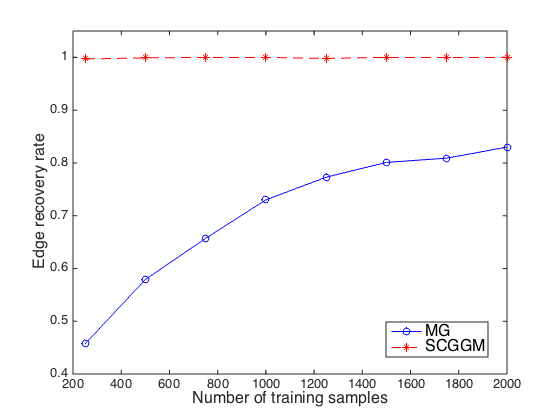
\includegraphics[width=3in]{figure/figure1}
  \caption[] {Edge recovery rate of MG and SCGGM on the synthetic dataset. Edge recovery rate of SCGGM is above $95\%$ for all training sample sizes and greater than that of MG.}
\end{figure}

Figure \ref{fig:syn_edge_rec} shows the accuracy of edge discovery of sparse CGGM and our method varying the number of samples used from 250 to 2000. The overall accuracy of sparse CGGM is greater than $97\%$ for all number of samples, but our method shows the lower accuracy  around $50\%$ on 250 samples and it grows to $80\%$ on increased number of samples. The accuracy is measured by averaging the accuracy of a single run over 10 times for both methods.

\subsection{More Synthetic Experiments}
As we believe the low performance of our model is due to the high simplicity and the small number of dimensions and parameters, we are planing to create a model with more dimensions and complexity and to train the models with less samples. We hope we can get results that our model is robust with relatively small size of the data as well as accurate in both prediction and edge discovery.

\subsection{Pre-processing SNPs-Gene Expression Data}
For exploring the eQTL mapping between SNPs and the expression rates of the related genes, we use the data from Human Liver Cohort(HLC) study \cite{schadt2008mapping} \footnote{The dataset is downloadable at \url{ https://www.synapse.org/\#!Synapse:syn4499}}. Out of 427 patients with more than 40,000 and more than 700,000 SNPs in the given data, we first extract 137 samples that contain both information on genotype and expression rates. To  focus on learning of the structure of the model rather than handling the huge dimension of this dataset, we focus on smaller subset of genes and expression rates as in the work of Sohn and coworker \cite{sohn2012joint}. We consider only expression rates whose variance is greater than 0.05 and SNPs on chromosome 6 with minor allele frequency greater than 0.01 and pair-wise correlation less than 0.1 to select genes that are not too biased to have major allele and not too related each other according to dbSNP\footnote{\url{http://www.ncbi.nlm.nih.gov/projects/SNP/}}. For a single nucleotide, where major allele is X and minor is Y, SNPs are encoded to categorical variables as XX = 0, XY = 1, YY = 2. SNPs are considered to be discrete variables with three states (0, 1, 2) and expression rates are to be continuous variables in our model.
 
At this point, the pre-processing of this HLC dataset is finished. After more analyses on the performance and the characteristics of our method, we will run our method on this data and report the results along with other baseline methods.

\section{Conclusion}
In this project, we adopt mixed graphical model for a better generative model in discovering the eQTL mapping in SNPs-gene networks. In synthetic experiments, our model shows lower performance in both prediction error and edge recovery rate than the baseline models due to the true model's simplicity. We will conduct more synthetic experiments on more complex synthetic model and real dataset from HLC study.



\nocite{*}
\bibliographystyle{icml2015}
\bibliography{final}

\end{document}


% This document was modified from the file originally made available by
% Pat Langley and Andrea Danyluk for ICML-2K. This version was
% created by Lise Getoor and Tobias Scheffer, it was slightly modified  
% from the 2010 version by Thorsten Joachims & Johannes Fuernkranz, 
% slightly modified from the 2009 version by Kiri Wagstaff and 
% Sam Roweis's 2008 version, which is slightly modified from 
% Prasad Tadepalli's 2007 version which is a lightly 
% changed version of the previous year's version by Andrew Moore, 
% which was in turn edited from those of Kristian Kersting and 
% Codrina Lauth. Alex Smola contributed to the algorithmic style files.  
